\chapter{Разработка метода решения задачи} \label{ch3}

% не рекомендуется использовать отдельную section <<введение>> после лета 2020 года
%\section{Введение} \label{ch3:intro}

Хорошим стилем является наличие введения к главе. Во введении может быть описана цель написания главы, а также приведена краткая структура главы. 
	
\section{Измерение инфракрасного излучения} \label{ch3:sec1}

Все объекты, температура которых превышает температуру абсолютного нуля излучают электромагнитное тепловое излучение. Согласно распределению длин волн, излучаемая энергия имеет зависимость от температуры поверхности объекта, которую можно описать законом излучения Планка:
\begin{equation} 
M(\lambda, T)=\frac{c_1 \lambda^{-5}}{\mathrm{e}^{c_2 / \lambda T}-1}
\end{equation} 
где $M(\lambda, T)$ величина излучения абсолютно черного тела. $c_1$ и $c_2$ первая и вторая константы излучения соответственно. $\lambda$ длина волны излучения и $T$ абсолютная температура черного тела. Когда $\exp \left(c_2 / \lambda T\right)>>1$, формулу Планка можно заменить следующей формулой смещения Вина:
\begin{equation} 
M_{\mathrm{b}}(\lambda, T)=c_1 \lambda^{-5} \mathrm{e}^{-c_2 / \lambda T}
\end{equation} 

Закон смещения Вина указывает на то, что чем выше температура объекта, тем короче длина волны его спектра излучения, и центральный пик смещается в сторону коротких волн. Однако излучаемая энергия, поступающая на чувствительную поверхность датчика, в реальных измерениях включает не только излучаемую энергию целевого объекта, но также энергию окружающих объектов и атмосферы. Поэтому спектральную излучательную способность поверхности целевого объекта можно выразить следующим образом:
\begin{equation} 
L_\lambda=\varepsilon_\lambda M_{\mathrm{b}}\left(\lambda, T_{\mathrm{obj}}\right)+\left(1-\alpha_\lambda\right) M_{\mathrm{b}}\left(\lambda, T_{\mathrm{sur}}\right)
\end{equation} 
где $\varepsilon_\lambda$ и $T_{\mathrm{obj}}$ излучательная способность и температура целевого объекта соответсвенно; $\varepsilon_\lambda M_b\left(\lambda, T_{\mathrm{obj}}\right)$ и $M_b(\lambda$, $T_{sur}$) это спектральная яркость целевого объекта и окружающей среды. $\alpha_\lambda$ поглощающая способность поверхности целевого объекта. $T_{\mathrm{sur}}$ температура окружающей среды.

Первый множитель в правой части уравнения (3.3) представляет собой спектральную яркость поверхности целевого объекта, а второй множитель — спектральную яркость окружающей среды, отраженную от целевого объекта. Излучение, действующее на систему измерения инфракрасного излучения, представлено на рисунке \ref{scheme}, основными источниками которого являются окружающая среда, объект и атмосфера. Это может быть выражено как:
\begin{equation} 
\begin{multlined}
E_\lambda=A_{\mathrm{obj}} d^{-2}\left[\tau_{\alpha \lambda} \varepsilon_\lambda M_{\mathrm{b}}\left(\lambda, T_{\mathrm{obj}}\right)+\tau_{\mathrm{a} \lambda}\left(1-\alpha_\lambda\right) \cdot M_{\mathrm{b}}\left(\lambda, T_{\mathrm{sur}}\right)+ \\ \varepsilon_{\alpha \lambda} M_{\mathrm{b}}\left(\lambda, T_{\mathrm{atm}}\right)\right]
\end{multlined}
\end{equation} 

\begin{figure}[ht!]
    \centering
    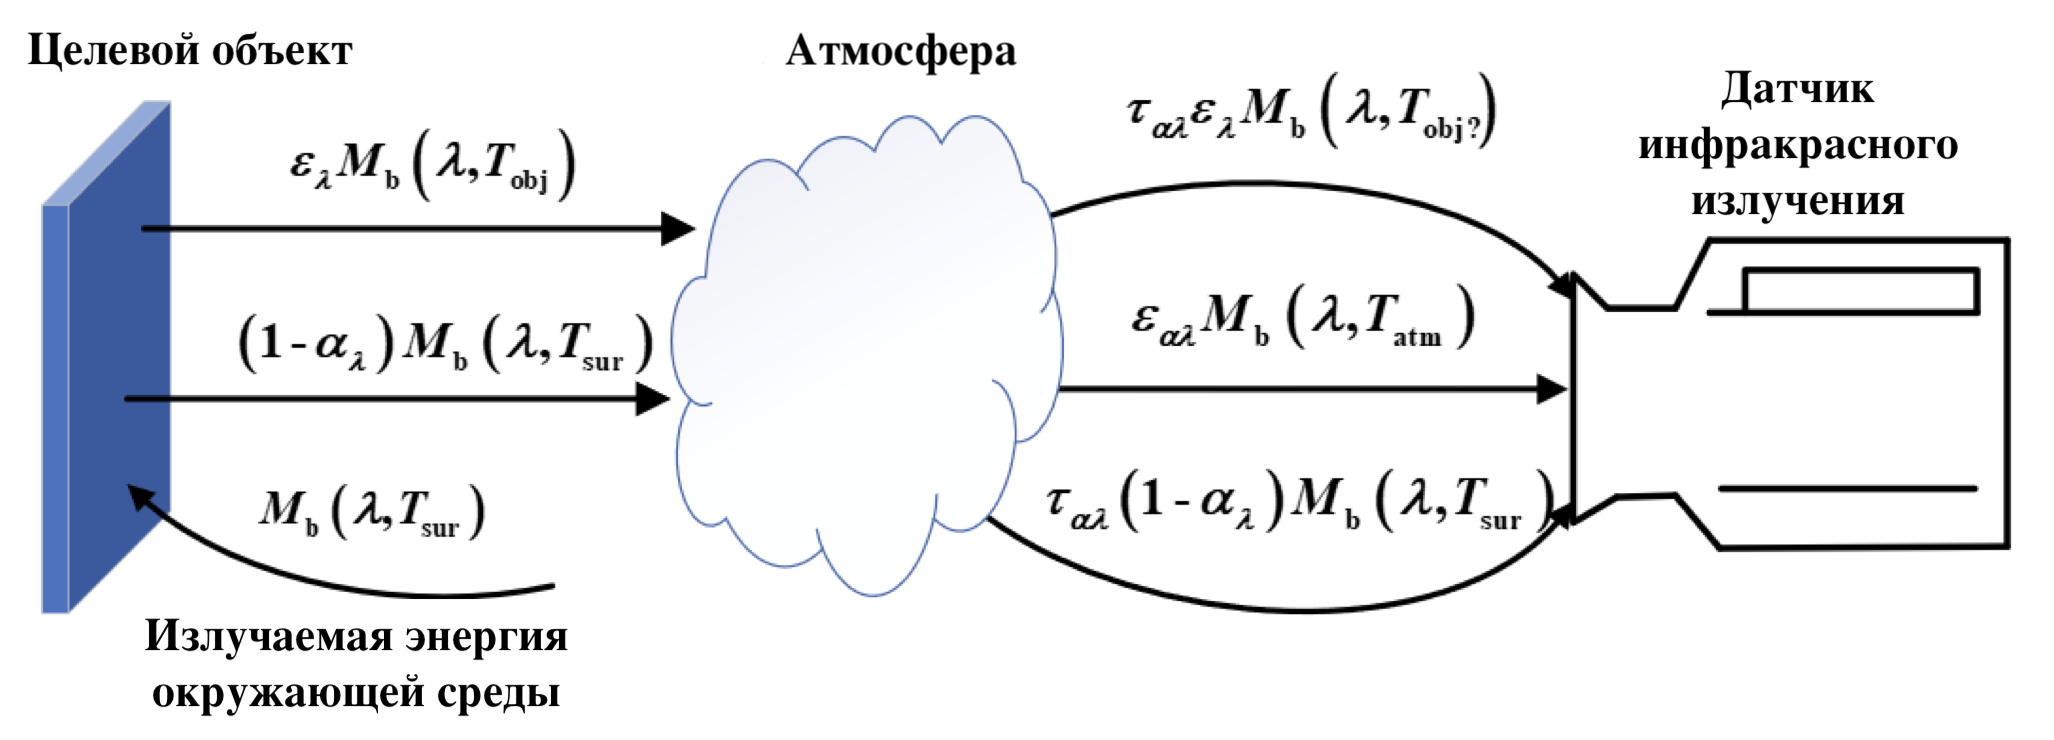
\includegraphics[width=0.8\linewidth]{my_folder/images/infr-scheme.png}
    \caption{Принципиальная схема получаемой энергии системы измерения инфракрасного излучения}
    \label{scheme}
\end{figure}
где $A_{\text{obj}}$ — видимая площадь целевого объекта, соответствующая минимальному углу тензора датчика инфракрасного изслучения, а $d$ — расстояние от целевого объекта до датчика инфракрасного излучения. В общем случае $\mathrm{A}_{\mathrm{obj}} d^{-2}$ является константой. $\tau_{\alpha \lambda}, \varepsilon_{\alpha \lambda} \mathrm{M}_{\mathrm{b}}\left(\lambda, T_{\mathrm{atm}}\right), \varepsilon_{\alpha \lambda}$ и $T_{\mathrm{atm}}$ — это спектральная пропускная способность, излучение, коэффициент излучения и температура атмосферы соответственно.

Полученная инфракрасная излучаемая энергия преобразуется датчиком в сигнал тока, то есть падающая инфракрасная излучаемая энергия интегрируется по полосе пропускания $\Delta \lambda$. Следовательно, зависимость между излучаемой энергией и током можно выразить следующим образом:
\begin{equation} 
I_0 = \int_{\Delta \lambda} A_{\mathrm{R}} R_\lambda E_\lambda \tau_{\mathrm{f}} \mathrm{d} \lambda
\end{equation} 
где $I_0$ — выходной сигнал тока датчика. $E_\lambda$ — освещенность радиации, полученная инфракрасной измерительной системой. $A_{\mathrm{R}}$ — площадь инфракрасной фокусирующей линзы. $R_\lambda$ — спектральная чувствительность инфракрасного датчика. $\tau_{\mathrm{f}}$ — пропускная способность оптической системы. Выходной ток можно преобразовать в сигнал напряжения через цепь преобразования I/V, что можно выразить следующим образом:
\begin{equation} 
\begin{multlined}
V_{\text {out }} = \int_{\Delta \lambda} R A_{\mathrm{obj}} d^{-2} A_{\mathrm{R}} \tau_f R_\lambda\left[\tau_{\alpha \lambda} \varepsilon_\lambda M_{\mathrm{b}}\left(\lambda, T_{\mathrm{obj}}\right) + \tau_{\alpha \lambda}(1 - \alpha_\lambda) M_{\mathrm{b}}\left(\lambda, T_{\text {sur}}\right) + \\ \varepsilon_{\alpha \lambda} M_{\mathrm{b}}\left(\lambda, T_{\mathrm{atm}}\right)\right] \mathrm{d} \lambda 
\end{multlined}
\end{equation}
где $R$ — нагрузка.

Уравнение (3.6) указывает, что существует множество факторов, влияющих на измерение инфракрасной температуры. На самом деле, эффективная площадь линзы, пропускная способность оптической системы и нагрузка определяются после спецификации аппаратного обеспечения системы измерения температуры. Когда $K = R A_{\mathrm{R}} \mathrm{T} \tau_{\mathrm{f}}$, уравнение (3.6) можно упростить следующим образом:
\begin{equation} 
\begin{multlined}
V_{\text {out }} = K A_{\mathrm{obj}} d^{-2} \int_{\Delta \lambda} R_\lambda\left[\tau_{\alpha \lambda} \varepsilon_\lambda \cdot M_{\mathrm{b}}\left(\lambda, T_{\mathrm{obj}}\right) + \tau_{\alpha \lambda}\left(1 - \alpha_\lambda\right) M_{\mathrm{b}}\left(\lambda, T_{\mathrm{sur}}\right) + \\\varepsilon_{\alpha \lambda} M_{\mathrm{b}}\left(\lambda, T_{\mathrm{atm}}\right)\right] \mathrm{д} \lambda
\end{multlined}
\end{equation} 

В таблице \ref{tab:equation7} представлено подробное описание переменных уравнения (3.7).

Из уравнения (3.7) видно, что точность измерений зависит от температуры окружающей среды, расстояния и угла измерения при определенной излучательной способности черного тела.

% Please add the following required packages to your document preamble:
% \usepackage{longtable}
% Note: It may be necessary to compile the document several times to get a multi-page table to line up properly
\begin{longtable}{|l|l|l|l|}
\caption{Описание переменных уравнения (3.7)}
\label{tab:equation7}\\
\hline
\multicolumn{1}{|c|}{Переменная}                & \multicolumn{1}{c|}{Описание}                                                                                                                                                  & \multicolumn{1}{c|}{Источник значения}                                                                                      & \multicolumn{1}{c|}{\begin{tabular}[c]{@{}c@{}}Единица \\ измерения\end{tabular}}                                           \\ \hline
\endhead
%
\( V_{\text{out}} \)                            & \begin{tabular}[c]{@{}l@{}}Выходное напряжение \\ на инфракрасном датчике\end{tabular}                                                                                         & \begin{tabular}[c]{@{}l@{}}Результат \\ измерений\end{tabular}                                                              & Вольт (V)                                                                                                                   \\ \hline
\( K \)                                         & \begin{tabular}[c]{@{}l@{}}Константа, определяющая \\ параметры оптической \\ системы инфракрасного \\ датчика: площадь линзы, \\ пропускная способность \\ линзы\end{tabular} & \begin{tabular}[c]{@{}l@{}}Задается \\ характеристиками \\ инфракрасного \\ детектора\end{tabular}                          & \begin{tabular}[c]{@{}l@{}}Безразмерная\\ величина\end{tabular}                                                             \\ \hline
\( A_{\text{obj}} \)                            & \begin{tabular}[c]{@{}l@{}}Видимая площадь \\ наблюдаемого \\ объекта\end{tabular}                                                                                             & \begin{tabular}[c]{@{}l@{}}Определяется \\ геометрией \\ объекта и \\ углом зрения \\ инфракрасного \\ датчика\end{tabular} & \begin{tabular}[c]{@{}l@{}}Квадратные \\ метры (\( \text{м}^2 \) )\end{tabular}                                             \\ \hline
\( d \)                                         & \begin{tabular}[c]{@{}l@{}}Расстояние от \\ наблюдаемого \\ объекта до \\ инфракрасного \\ датчика\end{tabular}                                                                & \begin{tabular}[c]{@{}l@{}}Измеряется в \\ экспериментальных \\ условиях\end{tabular}                                       & Метры (м)                                                                                                                   \\ \hline
\( \Delta \lambda \)                            & \begin{tabular}[c]{@{}l@{}}Спектральный \\ диапазон измерений\end{tabular}                                                                                                     & \begin{tabular}[c]{@{}l@{}}Задается \\ характеристиками \\ инфракрасного \\ датчика\end{tabular}                            & \begin{tabular}[c]{@{}l@{}}Микрометры \\ ( \( \mu \) m)\end{tabular}                                                        \\ \hline
\( R_\lambda \)                                 & \begin{tabular}[c]{@{}l@{}}Спектральная \\ чувствительность \\ инфракрасного \\ датчика\end{tabular}                                                                           & \begin{tabular}[c]{@{}l@{}}Задается \\ характеристиками \\ инфракрасного \\ датчика\end{tabular}                            & \begin{tabular}[c]{@{}l@{}}Безразмерная\\ величина\end{tabular}                                                             \\ \hline
\( \tau_{\alpha \lambda} \)                     & \begin{tabular}[c]{@{}l@{}}Спектральная \\ пропускная \\ способность \\ атмосферы\end{tabular}                                                                                 & \begin{tabular}[c]{@{}l@{}}Табличные или \\ экспериментальные\\ данные\end{tabular}                                         & \begin{tabular}[c]{@{}l@{}}Безразмерная\\ величина\end{tabular}                                                             \\ \hline
\( \varepsilon_\lambda \)                       & \begin{tabular}[c]{@{}l@{}}Излучательная \\ способность объекта\end{tabular}                                                                                                   & Табличные данные                                                                                                            & \begin{tabular}[c]{@{}l@{}}Безразмерная\\ величина\end{tabular}                                                             \\ \hline
\( M_{\mathrm{b}}(\lambda, T_{\mathrm{obj}}) \) & \begin{tabular}[c]{@{}l@{}}Спектральная плотность \\ излучения объекта при \\ температуре \( T_{\mathrm{obj}} \)\end{tabular}                                                  & \begin{tabular}[c]{@{}l@{}}Вычисляется по \\ закону Планка\end{tabular}                                                     & \begin{tabular}[c]{@{}l@{}}Ватты на \\ квадратный \\ метр на \\ микрометр \\ (Вт/\( \text{м}^2 \)/\( \mu \) м)\end{tabular} \\ \hline
\( M_{\mathrm{b}}(\lambda, T_{\mathrm{sur}}) \) & \begin{tabular}[c]{@{}l@{}}Спектральная плотность \\ излучения окружающей \\ среды при \\ температуре \( T_{\mathrm{sur}} \)\end{tabular}                                      & \begin{tabular}[c]{@{}l@{}}Вычисляется по \\ закону Планка\end{tabular}                                                     & \begin{tabular}[c]{@{}l@{}}Ватты на \\ квадратный \\ метр на \\ микрометр \\ (Вт/\( \text{м}^2 \)/\( \mu \) м)\end{tabular} \\ \hline
\( \tau_{\alpha \lambda}(1-\alpha_\lambda) \)   & \begin{tabular}[c]{@{}l@{}}Фактор отражения \\ излучения \\ окружающей среды\end{tabular}                                                                                      & \begin{tabular}[c]{@{}l@{}}Табличные или \\ экспериментальные\\ данные\end{tabular}                                         & \begin{tabular}[c]{@{}l@{}}Безразмерная\\ величина\end{tabular}                                                             \\ \hline
\( M_{\mathrm{b}}(\lambda, T_{\mathrm{atm}}) \) & \begin{tabular}[c]{@{}l@{}}Спектральная плотность \\ излучения атмосферы \\ при температуре \( T_{\mathrm{atm}} \)\end{tabular}                                                & \begin{tabular}[c]{@{}l@{}}Вычисляется по \\ закону Планка\end{tabular}                                                     & \begin{tabular}[c]{@{}l@{}}Ватты на \\ квадратный \\ метр на \\ микрометр \\ (Вт/\( \text{м}^2 \)/\( \mu \) м)\end{tabular} \\ \hline
\( \varepsilon_{\alpha \lambda} \)              & \begin{tabular}[c]{@{}l@{}}Спектральная излучательная \\ способность атмосферы\end{tabular}                                                                                    & \begin{tabular}[c]{@{}l@{}}Табличные или \\ экспериментальные\\ данные\end{tabular}                                         & \begin{tabular}[c]{@{}l@{}}Безразмерная\\ величина\end{tabular}                                                             \\ \hline
\end{longtable}

\section{Название параграфа} \label{ch3:sec2}

%\FloatBarrier % заставить рисунки и другие подвижные (float) элементы остановиться


\section{Выводы} \label{ch3:conclusion}

Текст выводов по главе \thechapter.


%% Вспомогательные команды - Additional commands
%
%\newpage % принудительное начало с новой страницы, использовать только в конце раздела
%\clearpage % осуществляется пакетом <<placeins>> в пределах секций
%\newpage\leavevmode\thispagestyle{empty}\newpage % 100 % начало новой страницы